\definecolor{bblue}{HTML}{4F81BD}
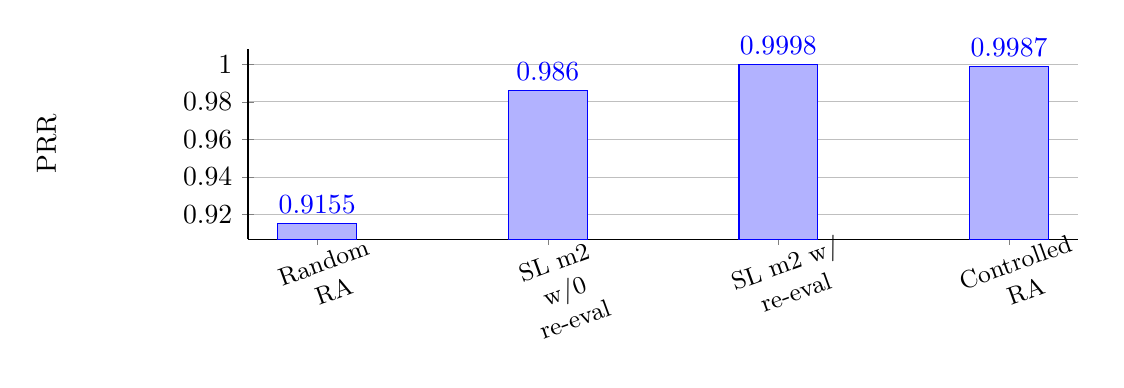
\begin{tikzpicture}
% \pgfplotscreateplotcyclelist{defaultCycle}{%
% ybar,%ybar legend,
% fill=customcolor,draw=black,opacity=1,thin,solid,mark=no,mark options=solid,\\%
% }
\begin{axis}
[
%    xbar, <--- comment this line 
    ybar,
    %cycle list name=defaultCycle,
    width=\columnwidth,
    height=4cm,
    %use units,
   % scale only axis,
    symbolic x coords={Random RA, SL m2 w/0 re-eval, SL m2 w/ re-eval, Controlled RA},
    xtick=data,
    nodes near coords,
    nodes near coords style={/pgf/number format/.cd,precision=5},
    %yticklabel style={/pgf/number format/fixed},,
    %ytick pos=left,
    axis y line*=left,
    xtick pos=bottom,
    axis x line*=bottom,
    %legend style={draw=none,at={(0,1.03)},anchor=south west},
    %legend columns=-1,
    xtick align=center,
    ytick align=center,
    % xtick distance=0.1,
    % ytick distance=,
    x tick label style ={font=\small,text width=1.5cm,anchor=north,rotate=20,align=center},
    y tick label style ={font=\normalsize,text width=2cm,anchor=east,rotate=0,align=right},
    %scaled y ticks=false,
    bar width=1cm,
    ymajorgrids,
    %xlabel=RA Techniques,
    ylabel=PRR,
    %title=\textbf{Team Points},
    ,
    ]
        \addplot+ table [x={x},y={y},meta index=2,col sep=semicolon] {
        x;  y;  z
        Random RA;  0.9155; 0
        SL m2 w/0 re-eval;  0.9860;  0
        SL m2 w/ re-eval;   0.9998;  0
        Controlled RA; 0.9987;  0
        };
      
\end{axis}
\end{tikzpicture}